\chapter{Capital Buffers, Cash Motion, and the Business of Keeping One's Word}

This chapter reads the Wall Street interviews as a compact lecture on the mechanics of wealth. The talk does not arrive as a formal derivation; it arrives as field evidence: a construction owner who says businesses fail because they are underfinanced, a financier who insists on saving, another who insists that money must move, and a trader who reduces business judgment to people, process, product, and profits. If we keep the sequence intact, a coherent structure appears. Wealth is not presented as a mystical trait. It is presented as buffer, motion, recovery, reputation, and selection.

\section{Numbers Before Theory}

The lecture begins in fragments. Someone has been broke multiple times. Someone else has been an entrepreneur for forty-nine years. A business has done roughly \$400 million in a single year. Another interviewee says he trades half a billion dollars of stock in a day, sits on five boards, and runs seven companies. Before any theory is offered, the lecture lays down scale:
\begin{align}
t_{\text{entrepreneur}} &\approx 49\,\text{yr},\\
R_{\max} &\approx 4.0\times 10^8\,\text{USD}\,\text{yr}^{-1},\\
V_{\text{trade}} &\approx 5.0\times 10^8\,\text{USD}\,\text{day}^{-1},\\
N_{\text{boards}} &= 5,\qquad N_{\text{companies}} = 7.
\end{align}
These are interview claims, not audited statements, but they are not dropped idly. The lecture wants the numbers on the table before it asks the real question: what do people around money seem to know that ordinary discourse obscures?

Then the governing question is made explicit. We are on Wall Street, and the experiment is to ask millionaires how they became wealthy and what financial freedom requires. The opening therefore functions as a teaser in the strict sense: scale comes first, law second.

\section{Scarcity, Refusal, and the Price of Advice}

Before the lecture gives us any durable answer, it gives us refusal. People are in a hurry, unwilling to stop, skeptical of the interruption. The point is not merely cinematic. Advice acquired under pressure is dense. We are not listening to polished memoir; we are extracting compressed operating rules.

This matters for the rhythm of the chapter. The first long answer feels earned because the lecture spends time showing us how hard it is to get a serious respondent. Persistence is part of the pedagogy. One keeps asking until a mechanism appears. The lecture is careful here: it does not jump directly into principles, because it wants us to feel the cost of obtaining them.

\section{Capital Buffers and Business Survival}

The first major mechanism arrives with the construction owner. The host frames the business problem bluntly: many firms do not survive five years. The reply is even blunter: they are underfinanced. There is luck in the world, the speaker says, but the safest way is to be well financed. At once the lecture stops being merely anecdotal and becomes structural.

We can capture the host's framing by the rough empirical claim
\begin{equation}
p_{\text{business fail by 5y}} \approx 0.8.
\end{equation}
Whether or not the number is exact is not the point. The point is that the interviewee's answer does not appeal to charisma, branding, or inspiration. It appeals to capital adequacy.

\begin{definition}
We shall call \(K_{\text{buffer}}\) the liquid capital available to keep a firm alive through ordinary operating burn and through the shocks that are certain to arrive but uncertain in size and timing.
\end{definition}

\paragraph{A first derivation.}
\begin{enumerate}
\item Let \(B\) denote the ordinary burn required to remain alive for one unit of time.
\item Let \(T\) denote the horizon over which the firm must survive before conditions improve, revenue catches up, or financing can be renewed.
\item Let \(S\) denote the extra reserve required by bad luck: delays, overruns, missed payments, legal friction, and all the other bumps along the road.
\item Ordinary survival costs \(BT\).
\item Shock-adjusted survival therefore costs \(BT+S\).
\end{enumerate}

\begin{proposition}[Capital buffer principle]
If a business faces ordinary burn \(B\) over horizon \(T\) and must reserve \(S\) for shocks, then the minimum survival condition is
\begin{equation}
K_{\text{buffer}} \ge BT + S.
\end{equation}
\end{proposition}

\begin{proof}
The firm must pay the ordinary carrying cost \(BT\) even if nothing goes wrong. Once we add the reserve \(S\) required by the predictable fact of unpredictability, the total required liquidity becomes \(BT+S\). If available liquid capital falls below that quantity, the firm may still survive by luck, but it is no longer protected against the very disturbances the speaker is warning us about.
\end{proof}

This first law explains why the lecture asks about class trajectory immediately afterward. The construction owner says he did not come from money. The desire was to create success for himself. But desire is not yet a buffer. The lecture therefore keeps both levels in play: aspiration on the one hand, capital adequacy on the other. One without the other is unstable.

The same speaker gives the sales corollary. In a competitive industry, he says, one sells by doing the right job. The delivered work is the best three-dimensional business card one can have. That line belongs here because it closes the loop: buffers keep the firm alive long enough to do the work; the work, if done correctly, becomes the advertisement that generates future work.

\section{Integrity, Clients, Family, and Risk}

The lecture does not leave the construction interview at the level of finance. It widens into operating constraints: be honest, keep the clients satisfied, put the family first, keep faith near the top of the list, and understand that early risk is easier when one has little to lose. The host's own recap makes the moral stakes unmistakable: if you do not keep your word in business, you have no business.

That sentence can be written as an update rule. It is not a theorem from the lecture; it is a companion formalization of its logic:
\begin{equation}
R_{t+1} = R_t + \alpha K_t - \beta B_t,
\end{equation}
where \(R_t\) is reputation, \(K_t\) counts kept commitments, and \(B_t\) counts broken ones. We should read \(\alpha\) and \(\beta\) qualitatively: promises kept add to the stock of trust; promises broken subtract from it, often more violently than the gains were accumulated.

The construction owner's remarks about clients and honesty are therefore not sentimental decoration. They are part of the production function of repeated business. In a one-shot transaction one may imagine cheating. In an actual operating life one compounds trust or one compounds its absence.

Risk also receives a careful placement. The lecture does not romanticize it abstractly. The speaker says risk felt easy because there was little to lose; if things failed, he could go back to his tools. In other words, risk tolerance is not a universal trait. It depends on the outside option.

\section{Saving, Deployment, and Time Ownership}

The next Wall Street interview narrows the frame from the firm to the person. The advice now comes in short, hard fragments: save every penny you can; when you are young you wrongly think money grows on trees; fear of failure is a primary motivator; avoid investing with friends and family; billionaires remove emotion from money; communication matters; truth matters; keeping one's word matters; and if one wants freedom, one should think in five- and ten-year plans rather than in a week's excitement.

What is striking is that this sequence does not stay at the level of thrift. The host pulls an entrepreneurial conclusion out of it: do not imagine that salaried dependence will automatically produce freedom. Buy back your time. Delegate. Work toward a position in which your life is not exhausted by the exchange of hours for wages. The lecture is now moving from money management to time ownership.

\subsection{Question \& Answer}

The lecture now presents a real tension. One speaker says, with great force, save every penny. Another, just ahead of us, will say with equal force that money has to keep moving. Are these contradictory rules?

They are contradictory only if we insist on using the same variable for two different functions of capital. The lecture is more intelligible if we separate reserve from deployment. Let \(s_t\) denote fresh saving and \(I_t\) denote capital actually deployed into productive motion. Then a minimal wealth dynamics reads
\begin{equation}
W_{t+1}=W_t+s_t+r_t I_t-L_t.
\end{equation}
Saving enters as capital formation. Motion enters through the return term \(r_t I_t\). Loss enters through \(L_t\).

In this form the tension dissolves. To save is not to worship idleness; it is to form the capital base from which choice becomes possible. To move money is not to despise reserve; it is to refuse sterility once a sufficient reserve exists. Setting \(I_t=0\) gives
\begin{equation}
W_{t+1}=W_t+s_t-L_t,
\end{equation}
which is safer than reckless speculation but powerless to compound through return. Setting \(s_t=0\) and overdeploying everything may produce return in the good state and fragility in the bad. The lecture's real answer is therefore two-layered: save for survival, deploy for growth.

\begin{figure}
\centering
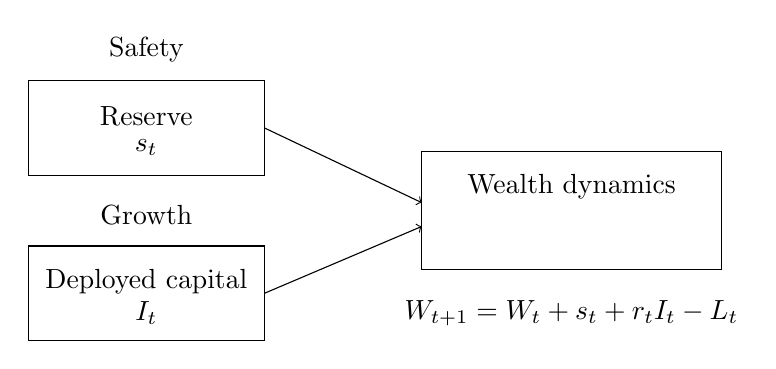
\begin{tikzpicture}[x=1cm,y=1cm]
\draw (0,0.3) rectangle (3,1.5);
\node at (1.5,1.05) {Reserve};
\node at (1.5,0.65) {\(s_t\)};
\node at (1.5,1.9) {Safety};

\draw (0,-1.8) rectangle (3,-0.6);
\node at (1.5,-1.05) {Deployed capital};
\node at (1.5,-1.45) {\(I_t\)};
\node at (1.5,-0.2) {Growth};

\draw (5,-0.9) rectangle (8.8,0.6);
\node at (6.9,0.15) {Wealth dynamics};

\draw[->] (3,0.9) -- (5,-0.05);
\draw[->] (3,-1.2) -- (5,-0.35);

\node at (6.9,-1.45) {\(W_{t+1}=W_t+s_t+r_t I_t-L_t\)};
\end{tikzpicture}
\caption{A transcript-based reconstruction of the two-layer capital rule. The lecture's tension is not between saving and investing as mutually exclusive doctrines, but between cash kept for endurance and capital deployed for growth.}
\end{figure}

\section{Loss, Recovery Time, and the Exchange Model}

The next interview pushes the lecture into its most abstract and most dangerous territory. The speaker says money must keep moving. It must not sit in the bank or under the mattress if the goal is growth. Then, abruptly, the lecture turns to personal wipeout: a divorce that destroyed wealth, the need to start over, and the insistence that the true issue is not loss by itself but recovery time.

That is the right place to introduce a second quantitative relation:
\begin{equation}
T_{\text{rec}} \approx \frac{L}{\dot W_{\text{rebuild}}},
\end{equation}
where \(L\) is the effective loss and \(\dot W_{\text{rebuild}}\) is the rate at which one can rebuild wealth, business position, or earning power. The lecture's verbal point is that the same loss has different meanings at different ages because the remaining horizon and the attainable rebuild rate are not constant. The transcript becomes garbled when it tries to give a numerical age example, but the structural idea is clear: path dependence enters through recovery time.

From here the talk turns from finance into exchange. Do not confuse socializing with networking. Every interaction should be examined as an exchange. What do I get? What do you get? Is there value here, or merely motion without substance? We can formalize this in the leanest possible way.

\begin{definition}
For an interaction between parties \(i\) and \(j\), define the exchange value
\begin{equation}
E_{ij}=G_{ij}-C_{ij},
\end{equation}
where \(G_{ij}\) is the gain extracted from the relation and \(C_{ij}\) is its cost in time, distraction, money, trust, or opportunity.
\end{definition}

Then the lecture's language about assets and liabilities can be stated as
\begin{equation}
E_{ij}>0 \Rightarrow \text{asset-like relation}, \qquad
E_{ij}<0 \Rightarrow \text{liability-like relation}.
\end{equation}

The inhale-exhale passage belongs here. The speaker moves from breathing to ecosystem barter: oxygen out, carbon dioxide back, then the trees reverse the transaction. He calls this contract and expand, contract and expand. We should be careful. This is not a literal scientific derivation. It is a transcript-based metaphor for reciprocal exchange. But it is not a bad metaphor. It says that every stable system alternates intake and output; pure intake suffocates it, and pure output empties it.

\begin{remark}
The breathing analogy is not presented as biology for its own sake. It is a rule of commercial and social orientation: whenever we enter a relation, we should ask what is actually being exchanged, and whether the rhythm of the exchange is sustainable.
\end{remark}

This same interview ends with the Einstein line about reality as a persistent illusion. In the lecture's logic, that remark is less a metaphysical thesis than a warning against naive literalism. Wealth, status, and disaster can all feel absolute in the moment. The speaker is trying to recover freedom by inserting distance between appearance and judgment.

\section{Screening Ideas and the Meaning of Rich}

After a brief promotional interruption, the lecture returns with a self-styled Einstein of Wall Street, and the tone changes. We are back inside a more orderly business vocabulary. The speaker emphasizes energy for the work, then warns that founders fall in love with an idea without asking whether it can actually survive. He invokes the familiar four-part screen: people, process, product, and profits.

We may package that screen as
\begin{equation}
\mathcal{S}(b)=\bigl(People(b),\,Process(b),\,Product(b),\,\Pi(b)\bigr).
\end{equation}

The lecture's point is not that these four entries can be maximized independently. Its point is that emotional attachment must be subordinated to examination. If the business cannot be profitable, cannot employ people, or cannot sustain a workable process, then love of the idea is not evidence in its favor. The same detachment is then carried over to trading: people fall in love with a trade, become trapped in ego, and refuse to take the profit or the loss with discipline.

This section also sharpens a distinction that has been waiting in the background the entire time. Money matters, but money is not the final quantity. The speaker refuses to make wealth identical with net worth. Family, meaningful work, the ability to inspire, and the ability to empower others all count toward being rich. Yet the lecture does not collapse into piety. It adds, very practically, that cash does equal freedom even if it does not equal happiness. One needs money, but one should not confuse it with the whole object.

Finally, the lecture asks how young people should choose an industry. The answer is observational. Walk around the school. Look at the phones, the shoes, the brands, the social media habits, the everyday loyalties. We are dealing with a consumer generation, and loyalty itself reveals the sectors where cultural energy and commercial demand meet. The notes should preserve the order here: first discipline, then screen, then a method of looking.

\section{Summary}

The lecture begins with scale and ends with discrimination. Between those two points it builds a surprisingly coherent chain. A business survives when it is buffered. A person advances when savings are disciplined, emotions are controlled, and time is progressively repurchased. Loss is governed not only by size but by recovery time. Relationships, like trades, must be judged by exchange rather than by sentiment alone. Reputation compounds when promises are kept. And profits, while necessary, do not exhaust the meaning of being rich.

If we keep the order of the lecture, the message becomes sharper. First endurance, then circulation; first truth, then scale; first selection, then compounding. Wealth is not presented as magic. It is presented as structure.